\documentclass[../VD.tex]{subfiles}

\externaldocument{../VD}

\begin{document}

\setcounter{chapter}{2}
\chapter{Subvariedades}\label{chap:subvd}

\section{Introducción}
\label{sec:subvd-intro}

\begin{definition}[name={subvariedad},label={def:subvd}]
  Dada una \(m\)-variedad \(M\), un subconjunto \(N \subseteq M\) se dice que es
  \emph{\(n\)-subvariedad} de \(M\) (\(n \leq m\)) si para todo \(p \in M\)
  existe una carta \((U,\varphi)\) de \(M\) con \(p \in U\) y tal que
  \begin{equation}
    \label{eq:subvd-cond}
    \varphi(U) \cap \RealSet^{m} = \varphi(U \cap N)
  \end{equation}

  Aquí, \(\RealSet^{n}\)
  se ve como el subespacio \(\RealSet^{n} \times \Set{0}^{m-n} \subseteq
  \RealSet^{m}\) de los puntos de \(\RealSet^{m}\) cuyas últimas \(m-n\)
  coordenadas son nulas.
\end{definition}

\begin{lemma}[label=lem:subvd-subset]
  Para todo \(A \subset U\) tenemos
  \begin{equation}
    \label{eq:lem-subvd-subset}
    \varphi(A) \cap \RealSet^{n} = \varphi(A \cap N)
  \end{equation}
\end{lemma}

\begin{proof}
  Si \(z \in \varphi(A) \cap \RealSet^{m} \subseteq \varphi(U) \cap \RealSet^{m}
  = \varphi(U \cap N)\), entonces existe \(p \in U \cap N\) con \(z =
  \varphi(p)\). Como \(z \in \varphi(A)\), \(p \in A\) y por ser inyectiva se
  tiene \(z \in \varphi(A \cap N)\).

  Si \(z \in \varphi(A \cap N) \subseteq \varphi(U \cap N) = \varphi(U) \cap
  \RealSet^{n}\), entonces \(z \in \RealSet^{n}\). Existe \(a \in A \cap N\) con
  \(\varphi(a) = z\), luego \(z \in \varphi(A) \cap \RealSet^{n}\). La otra
  contención es trivial.
\end{proof}

\begin{lemma}[label={lem:subvd-exists}]
  Para toda carta \((V,\psi)\) de \(M\) con \(p \in V\) se puede encontrar una
  carta \((W,\psi)\) con \(p \in W \subseteq V\) cumpliendo
  \eqref{eq:subvd-cond}.
\end{lemma}

\begin{proof}
  Sea \((U,\varphi)\) una carta de \(M\) cumpliendo \eqref{eq:subvd-cond}. Por
  la compatibilidad de cartas, \((W,\psi) = (U \cap V, \Restrict{\varphi}{U \cap
    V})\) es una carta de \(M\) con \(W \subseteq V\) y

  \begin{align*}
    \varphi(W) \cap \RealSet^{m}
    &= \varphi(U \cap V) \cap \RealSet^{m}\\
    &\overset{\mathclap{\eqref{eq:lem-subvd-subset}}}{=} \varphi(U \cap V \cap N)\\
    &= \varphi(W \cap N)
  \end{align*}
\end{proof}

\begin{lemma}[label={lem:subvd-vd}]
  Toda \(n\)-subvariedad \(N \subseteq M\) es una \(n\)-\nameref{def:vd}.
\end{lemma}

\begin{proof}
  Sabemos que dado \(p \in N\) existe una carta \((U_{p},\varphi_{p})\) de \(M\)
  con \(p \in U_{p}\) y \(\varphi_{p}(U_{p}) \cap \RealSet^{m} =
  \varphi_{p}(U_{p} \cap N)\).

  Entonces \((U_{p} \cap N, \Restrict{\varphi_{p}}{U_{p} \cap N}) \eqqcolon
  (W_{p}, \psi_{p})\) es un conjunto de cartas compatibles sobre \(N\).

  Notemos dos cosas:
  \begin{enumerate}
  \item \(\psi_{p}(W_{p}) = \varphi_{p}(U_{p} \cap N) = \varphi_{p}(U_{p}) \cap
    \RealSet^{n}\) es abierto de \(\RealSet^{n}\).
  \item  Si \(W_{p} \cap W_{q} \neq \emptyset\), entonces
    \begin{figure}[h]
      \centering
      \begin{tikzcd}[row sep=small]
        \mathllap{\psi_{q} \psi_{p}^{-1} \colon}
        \psi_{p}(W_{p} \cap W_{q})
        \ar[r] \ar[d,symbol={=}]
        & \psi_{q}(W_{p} \cap W_{q}) \ar[d,symbol={=}]\\
        \varphi_{p}(U_{p} \cap U_{q} \cap N) \ar[r] \ar[d, symbol={=}]
        & \varphi_{q}(U_{p} \cap U_{q} \cap N) \ar[d, symbol={=}]\\
        \mathllap{\varphi_{q} \varphi_{p}^{-1} \colon}
        \varphi_{p}(U_{p} \cap U_{q}) \cap \RealSet^{n}
        \ar[r]
        & \varphi_{q}(U_{p} \cap U_{q}) \cap \RealSet^{n}
      \end{tikzcd}
    \end{figure}

    es decir, \(\psi_{q} \psi_{p}^{-1}\) es restricción de
    \(\varphi_{q}\varphi_{p}^{-1}\) y por tanto diferenciable.
  \end{enumerate}

  Ahora aplicamos la \nameref{def:Lindelöff} a \(N \subseteq M\) y como \(N
  \subseteq \bigcup_{p \in N} U_{p}\), tenemos una cantidad numerable
  \(U_{p_{1}},\dots,U_{p_{n}},\dots\) con \(N \subseteq \bigcup_{n=1}^{\infty}
  U_{p_{n}}\), luego \(N = \bigcup_{n=1}^{\infty} W_{p_{n}}\), así que
  \(\mathcal{A} = \Set{(W_{p_{j}}, \psi_{p_{j}})}_{j \geq 1}\) es un atlas de
  \(N\).
\end{proof}

\begin{lemma}[label={lem:inclusion-inmersion}]
  La inclusión \(i \colon N \hookrightarrow M\) es una \nameref{def:inmersión}
  inyectiva.
\end{lemma}

\begin{proof}
  Obviamente \(i\) es inyectiva. Además es inmersión pues dado \(p \in N\), si
  \((U,\varphi)\) es una carta de \(M\) con \(p \in M\) cumpliendo la condición
  de \nameref{def:subvd} entonces \((U \cap N, \Restrict{\varphi}{U \cap N})\)
  es una carta con \(p \in U \cap N\) y
  \begin{figure}[h]
    \centering
    \begin{tikzcd}[column sep=small]
      U \cap N \ar[d, "\Restrict{\varphi}{U \cap N}"'] \ar[r, hook, "i"]
      & U \ar[rd, "\varphi"] \\
      \varphi(U \cap N) \ar[r, equal]
      &\varphi(U) \cap \RealSet^{n}
      \ar[r, "\overline{i}"', hook, dashed] & \varphi(U)
    \end{tikzcd}
  \end{figure}
  
  con \(\overline{i}\) la inclusión que obviamente tiene rango \(m\).
\end{proof}

\begin{example}
  Hay inmersiones inyectivas cuyas imágenes no son subvariedades. Supongamos \(M
  = \RealSet^{2}\) y \(N = \RealSet\) en la \cref{fig:inmersion-no-subvd}. En
  este caso \(U \cap N\) tiene forma de T, por lo que \(\varphi(U \cap N)\) no
  puede ser \(\varphi(U) \cap \RealSet^{m}\) porque la DIF-topología de \(N\) y
  la topología relativa de \(M\) no coinciden: para la topología relativa desde
  el punto \(p\) vemos una T, mientras que para la DIF-topología sólo se ve un
  intervalo, que no es homeomorfo a una T.
  \begin{figure}[h]
    \centering
    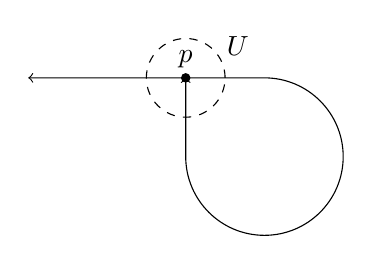
\begin{tikzpicture}[scale=2]
      \coordinate(p) at (0,0);
      \filldraw[black] (p) circle (0.75pt) node[above]{\(p\)};
      \draw[<->] (p) -- ++(0,-0.5) arc (-180:90:0.5) -- (-1,0);
      % \draw[<->] (p) .. controls (0,-1) and (1.5,0) .. (p) -- +(-1,0);
      \draw[dashed] (p) circle (0.25);
      \node[right] (ulabel) at (0.2,0.2) {\(U\)};
    \end{tikzpicture}
    \caption{Ejemplo de inmersión que no forma subvariedad}
    \label{fig:inmersion-no-subvd}
  \end{figure}
\end{example}

\begin{lemma}[label={lem:subvd-diftop}]
  Si \(N\) es subvariedad de \(M\), entonces la \nameref{def:diftop} de la
  estructura de variedad de \(N\) coincide con la topología relativa de la
  \nameref{def:diftop} de \(M\).
\end{lemma}

\begin{proof}
  Sea \(G \subseteq N\) abierto de la \nameref{def:diftop} de \(N\). Sea \(p \in
  G\) y sea \((U,\varphi)\) una carta de \(M\) con \(p \in U\) cumpliendo la
  propiedad de \nameref{def:subvd}. Entonces \(\varphi(G \cap U \cap N)\) es
  abierto de \(\varphi(U \cap N)\) y por tanto \(G \cap U \cap N\) es abierto de
  \(U \cap N\) (que es abierto de la topología relativa de \(N\) pues
  \(U\) es abierto de \(M\)).

  Así, \(G \cap U \cap N\) es abierto de \(N\), que es abierto de la topología
  relativa de \(N\) y \(p \in G \cap U \cap N \subseteq G\), por lo que \(G\) es
  abierto de la relativa.

  Ahora sea \(G \subseteq N\) abierto de la topología relativa, i.e. \(G =
  \Omega \cap N\) con \(\Omega\) abierto de la DIF-topología de \(M\).

  Para toda \((U,\varphi)\) carta de \(M\) con la propiedad de
  \nameref{def:subvd}, se tiene que \(\varphi(U) \cap \RealSet^{m} = \varphi(U
  \cap N)\). Entonces
  \begin{align*}
    \varphi(U \cap G)
    &= \varphi(U \cap N \cap G) = \varphi(U \cap \Omega \cap N)\\
    &= \varphi(U \cap \Omega) \cap \RealSet^{n}
  \end{align*}
  es abierto de \(\RealSet^{m}\) contenido en \(\varphi(U \cap N)\), así que
  \(G\) es abierto de la \nameref{def:diftop}.
\end{proof}

El siguiente resultado nos proporciona unan cantidad considerable de ejemplos de
subvariedades:

\begin{theorem}[label={thm:dim-inv-sub}]
  Sea \(f \colon M^{m} \to N^{n}\) una aplicación diferenciable y \(X^{k}
  \subseteq N^{n}\) una subvariedad. Supongamos que \(f\) es una
  \hyperref[def:inmersión]{submersión} en todos los puntos de \(f^{-1}(X)\).
  Entonces \(f^{-1}(X)\) es una \nameref{def:subvd} de dimensión \(m-n+k\).
\end{theorem}

\begin{proof}
  Sea \(p \in f^{-1}(X)\). Por las hipótesis podemos encontrar una carta
  \((W_{f(p)},\psi_{f(p)})\) de \(N\) tal que
  \(\psi_{f(p)}(\psi_{f(p)}(W_{f(p)}) \cap \RealSet^{n-k}) =
  \psi_{f(p)}(W_{f(p)}) \cap X\).

  Dada la carta \((W_{f(p)},\psi_{f(p)})\), como \(f\) es submersión en \(p\),
  podemos encontrar una carta \((U_{p},\varphi_{p})\) en \(M\) tal que
  \[
    \psi_{f(p)} \circ f \circ \varphi_{p}^{-1} \colon
    \varphi_{p}(U_{p}) \to \psi_{f(p)}(W_{f(p)})
  \]
  es la proyección \((x_{1},\dots,x_{m}) \mapsto (x_{1},\dots,x_{n})\) de las
  primeras \(n\) coordenadas.
  % Hay que ver la demostración del resultado de submersión

  Sea ahora \(\RealSet^{m - n + k} \subseteq \RealSet^{m}\) el subespacio donde las
  \(n-k\) coordenadas nulas están las últimas entre las \(n\) posiciones.

  Entonces
  \[
    U_{p} \cap f^{-1}(X) = \varphi_{p}^{-1}(\varphi_{p}(U_{p}) \cap \RealSet^{m-n+k})
  \]

  En efecto, si \(a \in U_{p}\) denotamos \(x_{1}(a),\dots,x_{m}(a)\) las
  funciones coordenadas de \(\varphi_{p}\) y si \(b \in W_{f(p)}\), denotamos
  \(y_{1}(b),\dots,y_{n}(b)\) las coordenadas de \(\psi_{f(p)}\).

  El término de la derecha son los \(a \in U_{p}\) con
  \[x_{n-k+1}(a) = \cdots = x_{n}(a) = 0\] mientras que los de la izquierda son
  aquellos \(a \in U_{p}\)tales que \(f(a) \in X\), i.e. \[y_{k+1}(f(a)) =
    \cdots = y_{n}(f(a)) = 0\]

  Veamos que ambos conjuntos coinciden. En efecto, si estamos en el primero,
  tenemos
  \begin{align*}
    (y_{1}(f(a)), \dots, y_{n}(f(a)))
    &= \psi_{f(p)} \circ f \circ \varphi_{p}^{-1} (x_{1}(a), \dots, x_{n-k}(a),0,\dots,0)\\
    &= x_{1}(a),\dots,x_{n-k}(a),0,\dots,0
  \end{align*}

  Luego \(y_{k+1}(f(a)) = \cdots = y_{n}(f(a)) = 0\), i.e. se cumple la segunda
  condición. Veamos ahora la contención contraria: si se cumple la segunda
  condición, entonces
  \begin{align*}
    (y_{1}(f(a)), \dots, y_{k}(f(a)),0,\dots,0)
    &= \psi_{f(p)} \circ f \circ \varphi_{p}^{-1} (x_{1}(a),\dots,x_{m}(a))\\
    &= (x_{1}(a),\dots,x_{n}(a))
  \end{align*}
  Luego \(x_{k+1}(a) = \cdots = x_{n}(a) = 0\).
\end{proof}

\begin{note}
  Hay referencias para las que una \nameref{def:subvd} es simplemente la imagen
  de una \nameref{def:inmersión} inyectiva. Y denominando \emph{subvariedad
    regular} a lo que aquí llamamos subvariedad.
\end{note}

\begin{example}
  Si \(N \subseteq M\) es una subvariedad compacta, entonces \(N\) es subespacio
  cerrado de \(M\). No siempre ocurre si \(N\) no es compacta. En el caso de una
  espiral centrada en el origen, con \(N = \RealSet\) y \(M = \RealSet^{2}\),
  \(N\) es una subvariedad no cerrada pues \({\Clausura{N}}^{\RealSet^{2}} = N \cup
  \Set{(0,0)}\).
\end{example}

\begin{example}
	\begin{itemize}
		\item \label{dim-sub-pto}Caso particular \( X=\{q\} \) y \( f \) es submersión en \( f^{-1}(q) \) entonces \( f^{-1}(q) \) es subvariedad de \textit{dim} \( m-n \)
		\item Sea \( f\colon \RealSet^n\to \RealSet \) definida como \( f(x_1,\ldots,x_n)= \sum x_i^2 \) es submersión en \( \RealSet^n-\{0\} \) con \( X= \{1\} \) entonces \( f^{-1}(1)=S^{n-1} \)
	\end{itemize}
\end{example}

\begin{lemma}
	Sea \( f\colon M^m\to N^n \) submersión en \( p \). Para toda carta \( (W,\psi) \) de \( N \) con \( f(p)\in W \) se pueden encontrar cartas \( (U_0,\varphi_0) \) en \( M \) y \( (W_0,\psi_{0}) \) en \( N \) con \( p\in U_0 \), \( f(U_0)\subseteq W_0\subseteq W \) y \( \psi_0=\Restrict{\psi}{W_0} \)  tales que:
	\[
	\varphi_0(U_0)=\psi_{0}(W_0)\times \Omega
	\]
	donde \( \Omega \) es un abierto de \( \RealSet^{n-m} \). Además el siguiente diagrama es conmutativo
	\begin{figure}[h]
		\centering
		\begin{tikzcd}
		U_0 \arrow[r, "f"] \arrow[d, "\varphi_{0}"']
		& W_0 \arrow[d, "\psi_{0}"] \\
		\varphi_0(U_0) \arrow[r, "\psi_0\circ f\circ \varphi^{-1}" ']
		& \psi_0(W_0)
		\end{tikzcd}
		\caption{Diagrama submersión}
		\label{fig:sub}
	\end{figure}
\end{lemma}

\section{Incrustaciones}
\label{sec:incrustaciones}

\begin{definition}[name={incrustación},label={def:incrustación}]
  Una aplicación diferenciable \(f \colon M \to N\) se dice \emph{incrustación}
  (\emph{embedding}) si es inmersión inyectiva y la DIF-topología de estructura
  diferenciable de \(f(M)\) inducida por \(f \colon M \to f(M)\) coincide con la
  relativa de \(M\)
\end{definition}

\begin{theorem}[name={Whitney},label={thm:Whitney}]
  Toda \(m\)-variedad de \(M\) admite una \nameref{def:incrustación} de \(f
  \colon M \to \RealSet^{2m+1}\) tal que \(f(M)\) es subvariedad.
\end{theorem}

El \hyperref[thm:Whitney]{teorema de Whitney} nos dice que la teoría de
variedades se puede reducir a una teoría de subvariedades euclídeas. Pero como
no siempre tenemos a mano una \nameref{def:inmersión} explícita, seguimos
trabajando ``dentro'' de la variedad sin un ``mundo exterior'' para verla desde
fuera.

\begin{lemma}[name={propiedades de la incrustación},label={lem:incrust-prop}]
  Si \(f \colon M \to N\) es incrustación,
  \begin{enumerate}
  \item \(f(M)\) es subvariedad. \label{lem:incrust-prop.1}
  \item La estructura de subvariedad coincide con la inducida por \(f\). \label{lem:incrust-prop.2}
  \item \(f\) es difeomorfismo. \label{lem:incrust-prop.3}
  \end{enumerate}
\end{lemma}

\begin{proof}\item
  \begin{subproof}[\ref{lem:incrust-prop.1}]
    Debemos probar que para todo \(p \in f(M)\) existe una carta de
    \((U,\varphi)\) de \(p\) en \(N\) con \(p \in U\) y \(\varphi(U) \cap
    \RealSet^{m} = f(M) \cap \varphi(U)\). Aquí, \(\RealSet^{m} \equiv
    \RealSet^{n} \times \Set{\cdot} \subseteq \RealSet^{n}\).
    
    Como \(f\) es \nameref{def:inmersión}, sabemos que para \(q\) con \(f(q) =
    p\) existen cartas \((\Omega,\rho)\) de \(M\) y \((U,\varphi)\) de \(N\)
    tales que \(q \in \Omega\), \(f(\Omega) \subseteq U\) con el diagrama de la
    \cref{fig:inmersion-cd} (p.~\pageref{fig:inmersion-cd}).

    Así, \(\varphi f \rho^{-1}(\rho\Omega) = \varphi f(\Omega) = \rho(\Omega)
    \times \Set{0}\) es un abierto de \(\RealSet^{m}\) contenido en
    \(\varphi(U)\). Por tanto, podemos encontrar un abierto \(G\) de
    \(\RealSet^{n}\) con \(G \cap \RealSet^{m} = \varphi f(\Omega)\).

    Por otro lado, \(f(\Omega)\) es un abierto de \(f(M)\) y por hipótesis, \(W
    \subseteq N\) abierto con \(W \cap f(M) = f(\Omega)\).

    Sea \(V = \varphi^{-1}(G) \cap W \subseteq U \cap W\) abierto de \(N\).
    Ahora consideramos la carta \((V,\varphi_{0})\), con \(\varphi_{0} =
    \Restrict{\varphi}{V}\).
    Tenemos \(\varphi(V)\ \cap \RealSet^{m} = \varphi(V \cap f(M))\).

    Si \(z \in \varphi(V) \cap \RealSet^{m}\), entonces \(z = \varphi(a)\) con
    \(a \in V = \varphi^{-1}(G) \cap W\). Por tanto, \(z = \varphi(a) \in G \cap
    \RealSet^{m} = \varphi(f(\Omega)) \subseteq \varphi(V \cap f(M))\), pues
    \(f(\Omega) \subseteq V = \varphi^{-1}(G) \cap W\).

    Recíprocamente, si \(z \in \varphi(V \cap f(M))\), entonces \(z =
    \varphi(a)\) con \(a \in V \cap f(M) = \varphi^{-1}(G) \cap W \cap f(M)
    \subseteq f(\Omega)\), luego \(z = \varphi(a) \in \varphi f(\Omega) = G
    \cap\RealSet^{m}\), luego \(z \in \RealSet^{m}\) y \(z = \varphi(a) \in
    \varphi(V)\).

    % TODO: añadir esquema de (T-3).8
  \end{subproof}

  \begin{subproof}[\ref{lem:incrust-prop.3}]
    Es obvia por la teoría anterior % TODO: añadir referencia
  \end{subproof}
\end{proof}

\begin{lemma}
  Si \(f \colon M \to N\) es una \nameref{def:inmersión} inyectiva y \(f(M)\) es
  una \nameref{def:subvd} de \(N\) con la estructura inducida por \(f\),
  entonces \(f\) es \nameref{def:incrustación}.
\end{lemma}

\begin{proof}
  Toda \nameref{def:subvd} de \(N\) cumple que su \nameref{def:diftop} es la
  relativa de la de \(N\).
\end{proof}

\begin{example}
  Naturalmente hay muchas \hyperref[def:inmersión]{inmersiones} inyectivas o
  \hyperref[def:incrustación]{incrustaciones} de una misma variedad. Por
  ejemplo, todos los nudos son incrustaciones de \(S^{1}\) en \(\RealSet^{3}\).
  % TODO: añadir figuras con al menos un nudo no trivial.

  Por otra parte, una recta y una espiral son dos incrustaciones de \(\RealSet\)
  en \(\RealSet^{2}\).
\end{example}

\begin{definition}[{name=[equivalentes]{incrustaciones equivalentes}},
  label={def:incrust-equiv}]
  Dos \hyperref[def:incrustación]{incrustaciones} \(f,g \colon M \to N\) se
  dicen \emph{equivalentes} si existe un difeomorfismo \(h \colon N \to N\) tal
  que \(h \circ f = g\).
\end{definition}

\section{Ejercicios Interesantes de la Relación 3}

\begin{Exercise}[number=1]\label{ex:3.1}
Si \(M\) es una variedad compacta, probar que toda inmersión inyectiva \(f\colon M \to N\) es incrustación.
\end{Exercise}

\begin{Answer}[number=1]
En primer lugar recordemos que en un espacio topológico cualquiera si tenemos una función \(f\colon X\to Y\) biyectiva con \(X\) compacto y Hausdorff e \(Y\) Hausdorff, entonces \(f\) es homeomorfismo.

Si aplicamos este resultado a \(\tilde{f}=\Restrict{f}{M}\) tenemos que
\[\tilde{f}\colon(M,\text{topología natural})\to(f(M),\text{topología relativa})
\]
cumple las hipótesis y por tanto \(\tilde{f}\) es homeomorfismo. Esto significa que ambas topologías son equivalentes. 
\end{Answer}

\begin{Exercise}[number=2]
Probar que el "ocho" con cualquiera de las dos estructuras vistas en %\nameref{ex:1.4} NO SE SI HAY REF DE ESE EJERCICIO
es la imagen de una inmersión inyectiva de \(\RealSet\) en \(\RealSet ^2\). ¿Puede ser la imagen de una incrustación.
\end{Exercise}

\begin{Answer}[number=2]
%Idea de resolución
Parametrizamos la curva como \(f(t)=(\sin(t),\sin(2t)\) claramente inyectiva y \(f'(t)=(\cos(t),2\cos(2t)\neq 0\) que prueba el carácter de inmersión. Pero la topología relativa da problemas en el punto de cruce.
\end{Answer}

\begin{Exercise}[number=5]
Sean \(M_0\subseteq M\) y \(N_0\subseteq N\) subvariedades. Probar que \(M_0\times N_0\) es subvariedad de \(M\times N\).
\end{Exercise}

\begin{Answer}[number=5]
Escribimos la definición de subvariedad en cada caso:
\begin{itemize}
	\item \(\exists (U,\varphi)\) carta de \(M\) con \(p\in U\) tal que \(\varphi(U\cap M_0=\varphi(U)\cap \RealSet^k)\) pudiendo escribir \(\RealSet^k\) como \(\RealSet^k\times \{0\}\subseteq \RealSet ^m\).
		\item \(\exists (W,\psi)\) carta de \(N\) con \(q\in U\) tal que \(\psi(W\cap N_0=\psi(W)\cap \RealSet^s)\) pudiendo escribir \(\RealSet^s\) como \(\RealSet^s\times \{0\}\subseteq \RealSet ^s\)
\end{itemize}
Luego \((U\times W,\varphi\times \psi)\) es carta de \(M\times N\) con \((p,q)\in U\times W\). Basta ver que ocurre con la imagen por \(\varphi\times \psi\)
\begin{align*}
(\varphi\times \psi )((U\times W) \cap & (M_0\times N_0))=\varphi(U\cap M_0)\times \psi(W\cap N_0)\\
&=(\varphi(U)\cap \RealSet^k)\times (\psi(W)\cap \RealSet^s)\\
&=(\varphi(U)\times \psi(W))\cap (\RealSet^k\times\{0\}\:\mathbf{\times}\:\RealSet^s\times \{0\})
\end{align*}
\end{Answer}

\begin{Exercise}[number=12]
Para cada \(a\in \RealSet\), sea \(M_a=\{(x,y)\in\RealSet^2\colon y² =x(x-1)(x-a)\}\).
\begin{enumerate}
\item Usando la aplicación adecuada \(f_a\colon \RealSet^2\to \RealSet\), para cada \(a\), probar que \(M_a\) es subvariedad incrustada de \(\RealSet^2\) salvo posiblemente para \(a=0,1\).
\item Probar que, también para \(a=0\), \(M_0\) sigue siendo una subvariedad, pero \(M_1\) no lo es.
\item Dar una estructura diferenciable sobre \(M_1\) que la haga imagen de una variedad por una inmersión inyectiva.
\end{enumerate}
\end{Exercise}

\begin{Answer}[number=12]
\begin{enumerate}
\item Definimos la función como
\begin{align*}
f_a\colon &\RealSet^2\to \RealSet\\
&(x,y)\mapsto y^2-x(x-1)(x-a)
\end{align*}
e imponemos que sea subvariedad incrustada en la matriz Jacobiana (en este caso un vector)
\[
(-(x-1)(x-a)-x(x-a)-x(x-1),2y)
\]
que para tener rango nulo ha de cumplirse el sistema
\[
\left\{
	\begin{array}{ll}
	y=0 & \\
	x=0=a & \text{ó} x=1=a
	\end{array}
\right.
\]
\item En el caso de \(a\neq 0,1\) el rango es \(1\), por lo que \(dim(M_a)=1\).\\
Para \(a=0\) la subvariedad es \(M_0=\{(x,y)\colon y^2=x^2(x-1)\}\) que salvo en el \((0,0)\) se puede ver que de hecho es homeomorfo a \(\RealSet\) %TODO: Incluir imagen.\\
Para \(a=1\) tenemos \(M_1=\{(x,y)\colon y^2=x(x-1)^2\}\) que la curva se corta a si misma. %TODO: incluir imagen
\item Para dotar a \(M_1\) de estructura diferenciable basta seguir el procedimiento para el "ocho".
\end{enumerate}
\end{Answer}

\end{document}

%%% Local Variables:
%%% TeX-master: "../VD"
%%% End: